\documentclass[12pt]{article}

%packages
%\usepackage{latexsym}
\usepackage{graphicx}
\usepackage{color}
\usepackage{amsmath}
\usepackage{dsfont}
\usepackage{placeins}
\usepackage{amssymb}
\usepackage{wasysym}
\usepackage{abstract}
\usepackage{hyperref}
\usepackage{etoolbox}
\usepackage{datetime}
\usepackage{xcolor}
\usepackage{wrapfig}
\usepackage{alphalph}
%\usepackage[singlelinecheck=false]{caption}
\settimeformat{ampmtime}

%\usepackage{pstricks,pst-node,pst-tree}

%\usepackage{algpseudocode}
%\usepackage{amsthm}
%\usepackage{hyperref}
%\usepackage{mathrsfs}
%\usepackage{amsfonts}
%\usepackage{bbding}
%\usepackage{listings}
%\usepackage{appendix}
\usepackage[margin=1in]{geometry}
%\geometry{papersize={8.5in,11in},total={6.5in,9in}}
%\usepackage{cancel}
%\usepackage{algorithmic, algorithm}

\makeatletter
\def\maxwidth{ %
  \ifdim\Gin@nat@width>\linewidth
    \linewidth
  \else
    \Gin@nat@width
  \fi
}
\makeatother

\definecolor{fgcolor}{rgb}{0.345, 0.345, 0.345}
\newcommand{\hlnum}[1]{\textcolor[rgb]{0.686,0.059,0.569}{#1}}%
\newcommand{\hlstr}[1]{\textcolor[rgb]{0.192,0.494,0.8}{#1}}%
\newcommand{\hlcom}[1]{\textcolor[rgb]{0.678,0.584,0.686}{\textit{#1}}}%
\newcommand{\hlopt}[1]{\textcolor[rgb]{0,0,0}{#1}}%
\newcommand{\hlstd}[1]{\textcolor[rgb]{0.345,0.345,0.345}{#1}}%
\newcommand{\hlkwa}[1]{\textcolor[rgb]{0.161,0.373,0.58}{\textbf{#1}}}%
\newcommand{\hlkwb}[1]{\textcolor[rgb]{0.69,0.353,0.396}{#1}}%
\newcommand{\hlkwc}[1]{\textcolor[rgb]{0.333,0.667,0.333}{#1}}%
\newcommand{\hlkwd}[1]{\textcolor[rgb]{0.737,0.353,0.396}{\textbf{#1}}}%

\usepackage{framed}
\makeatletter
\newenvironment{kframe}{%
 \def\at@end@of@kframe{}%
 \ifinner\ifhmode%
  \def\at@end@of@kframe{\end{minipage}}%
  \begin{minipage}{\columnwidth}%
 \fi\fi%
 \def\FrameCommand##1{\hskip\@totalleftmargin \hskip-\fboxsep
 \colorbox{shadecolor}{##1}\hskip-\fboxsep
     % There is no \\@totalrightmargin, so:
     \hskip-\linewidth \hskip-\@totalleftmargin \hskip\columnwidth}%
 \MakeFramed {\advance\hsize-\width
   \@totalleftmargin\z@ \linewidth\hsize
   \@setminipage}}%
 {\par\unskip\endMakeFramed%
 \at@end@of@kframe}
\makeatother

\definecolor{shadecolor}{rgb}{.77, .77, .77}
\definecolor{messagecolor}{rgb}{0, 0, 0}
\definecolor{warningcolor}{rgb}{1, 0, 1}
\definecolor{errorcolor}{rgb}{1, 0, 0}
\newenvironment{knitrout}{}{} % an empty environment to be redefined in TeX

\usepackage{alltt}
\usepackage[T1]{fontenc}

\newcommand{\qu}[1]{``#1''}
\newcounter{probnum}
\setcounter{probnum}{1}

%create definition to allow local margin changes
\def\changemargin#1#2{\list{}{\rightmargin#2\leftmargin#1}\item[]}
\let\endchangemargin=\endlist 

%allow equations to span multiple pages
\allowdisplaybreaks

%define colors and color typesetting conveniences
\definecolor{gray}{rgb}{0.5,0.5,0.5}
\definecolor{black}{rgb}{0,0,0}
\definecolor{white}{rgb}{1,1,1}
\definecolor{blue}{rgb}{0.5,0.5,1}
\newcommand{\inblue}[1]{\color{blue}#1 \color{black}}
\definecolor{green}{rgb}{0.133,0.545,0.133}
\newcommand{\ingreen}[1]{\color{green}#1 \color{black}}
\definecolor{yellow}{rgb}{1,1,0}
\newcommand{\inyellow}[1]{\color{yellow}#1 \color{black}}
\definecolor{orange}{rgb}{0.9,0.649,0}
\newcommand{\inorange}[1]{\color{orange}#1 \color{black}}
\definecolor{red}{rgb}{1,0.133,0.133}
\newcommand{\inred}[1]{\color{red}#1 \color{black}}
\definecolor{purple}{rgb}{0.58,0,0.827}
\newcommand{\inpurple}[1]{\color{purple}#1 \color{black}}
\definecolor{backgcode}{rgb}{0.97,0.97,0.8}
\definecolor{Brown}{cmyk}{0,0.81,1,0.60}
\definecolor{OliveGreen}{cmyk}{0.64,0,0.95,0.40}
\definecolor{CadetBlue}{cmyk}{0.62,0.57,0.23,0}

%define new math operators
\DeclareMathOperator*{\argmax}{arg\,max~}
\DeclareMathOperator*{\argmin}{arg\,min~}
\DeclareMathOperator*{\argsup}{arg\,sup~}
\DeclareMathOperator*{\arginf}{arg\,inf~}
\DeclareMathOperator*{\convolution}{\text{\Huge{$\ast$}}}
\newcommand{\infconv}[2]{\convolution^\infty_{#1 = 1} #2}
%true functions

%%%% GENERAL SHORTCUTS

%shortcuts for pure typesetting conveniences
\newcommand{\bv}[1]{\boldsymbol{#1}}

%shortcuts for compound constants
\newcommand{\BetaDistrConst}{\dfrac{\Gamma(\alpha + \beta)}{\Gamma(\alpha)\Gamma(\beta)}}
\newcommand{\NormDistrConst}{\dfrac{1}{\sqrt{2\pi\sigma^2}}}

%shortcuts for conventional symbols
\newcommand{\tsq}{\tau^2}
\newcommand{\tsqh}{\hat{\tau}^2}
\newcommand{\sigsq}{\sigma^2}
\newcommand{\sigsqsq}{\parens{\sigma^2}^2}
\newcommand{\sigsqovern}{\dfrac{\sigsq}{n}}
\newcommand{\tausq}{\tau^2}
\newcommand{\tausqalpha}{\tau^2_\alpha}
\newcommand{\tausqbeta}{\tau^2_\beta}
\newcommand{\tausqsigma}{\tau^2_\sigma}
\newcommand{\betasq}{\beta^2}
\newcommand{\sigsqvec}{\bv{\sigma}^2}
\newcommand{\sigsqhat}{\hat{\sigma}^2}
\newcommand{\sigsqhatmlebayes}{\sigsqhat_{\text{Bayes, MLE}}}
\newcommand{\sigsqhatmle}[1]{\sigsqhat_{#1, \text{MLE}}}
\newcommand{\bSigma}{\bv{\Sigma}}
\newcommand{\bSigmainv}{\bSigma^{-1}}
\newcommand{\thetavec}{\bv{\theta}}
\newcommand{\thetahat}{\hat{\theta}}
\newcommand{\thetahatmle}{\hat{\theta}_{\mathrm{MLE}}}
\newcommand{\thetavechatmle}{\hat{\thetavec}_{\mathrm{MLE}}}
\newcommand{\muhat}{\hat{\mu}}
\newcommand{\musq}{\mu^2}
\newcommand{\muvec}{\bv{\mu}}
\newcommand{\muhatmle}{\muhat_{\text{MLE}}}
\newcommand{\lambdahat}{\hat{\lambda}}
\newcommand{\lambdahatmle}{\lambdahat_{\text{MLE}}}
\newcommand{\etavec}{\bv{\eta}}
\newcommand{\alphavec}{\bv{\alpha}}
\newcommand{\minimaxdec}{\delta^*_{\mathrm{mm}}}
\newcommand{\ybar}{\bar{y}}
\newcommand{\xbar}{\bar{x}}
\newcommand{\Xbar}{\bar{X}}
\newcommand{\phat}{\hat{p}}
\newcommand{\Phat}{\hat{P}}
\newcommand{\Zbar}{\bar{Z}}
\newcommand{\iid}{~{\buildrel iid \over \sim}~}
\newcommand{\inddist}{~{\buildrel ind \over \sim}~}
\newcommand{\approxdist}{~{\buildrel approx \over \sim}~}
\newcommand{\equalsindist}{~{\buildrel d \over =}~}
\newcommand{\loglik}[1]{\ell\parens{#1}}
\newcommand{\thetahatkminone}{\thetahat^{(k-1)}}
\newcommand{\thetahatkplusone}{\thetahat^{(k+1)}}
\newcommand{\thetahatk}{\thetahat^{(k)}}
\newcommand{\half}{\frac{1}{2}}
\newcommand{\third}{\frac{1}{3}}
\newcommand{\twothirds}{\frac{2}{3}}
\newcommand{\fourth}{\frac{1}{4}}
\newcommand{\fifth}{\frac{1}{5}}
\newcommand{\sixth}{\frac{1}{6}}

%shortcuts for vector and matrix notation
\newcommand{\A}{\bv{A}}
\newcommand{\At}{\A^T}
\newcommand{\Ainv}{\inverse{\A}}
\newcommand{\B}{\bv{B}}
\newcommand{\K}{\bv{K}}
\newcommand{\Kt}{\K^T}
\newcommand{\Kinv}{\inverse{K}}
\newcommand{\Kinvt}{(\Kinv)^T}
\newcommand{\M}{\bv{M}}
\newcommand{\Bt}{\B^T}
\newcommand{\Q}{\bv{Q}}
\newcommand{\Qt}{\Q^T}
\newcommand{\R}{\bv{R}}
\newcommand{\Rt}{\R^T}
\newcommand{\Z}{\bv{Z}}
\newcommand{\X}{\bv{X}}
\newcommand{\Xsub}{\X_{\text{(sub)}}}
\newcommand{\Xsubadj}{\X_{\text{(sub,adj)}}}
\newcommand{\I}{\bv{I}}
\newcommand{\Y}{\bv{Y}}
\newcommand{\sigsqI}{\sigsq\I}
\renewcommand{\P}{\bv{P}}
\newcommand{\Psub}{\P_{\text{(sub)}}}
\newcommand{\Pt}{\P^T}
\newcommand{\Pii}{P_{ii}}
\newcommand{\Pij}{P_{ij}}
\newcommand{\IminP}{(\I-\P)}
\newcommand{\Xt}{\bv{X}^T}
\newcommand{\XtX}{\Xt\X}
\newcommand{\XtXinv}{\parens{\Xt\X}^{-1}}
\newcommand{\XtXinvXt}{\XtXinv\Xt}
\newcommand{\XXtXinvXt}{\X\XtXinvXt}
\newcommand{\x}{\bv{x}}
\newcommand{\onevec}{\bv{1}}
\newcommand{\oneton}{1, \ldots, n}
\newcommand{\yoneton}{y_1, \ldots, y_n}
\newcommand{\yonetonorder}{y_{(1)}, \ldots, y_{(n)}}
\newcommand{\Yoneton}{Y_1, \ldots, Y_n}
\newcommand{\iinoneton}{i \in \braces{\oneton}}
\newcommand{\onetom}{1, \ldots, m}
\newcommand{\jinonetom}{j \in \braces{\onetom}}
\newcommand{\xoneton}{x_1, \ldots, x_n}
\newcommand{\Xoneton}{X_1, \ldots, X_n}
\newcommand{\xt}{\x^T}
\newcommand{\y}{\bv{y}}
\newcommand{\yt}{\y^T}
\renewcommand{\c}{\bv{c}}
\newcommand{\ct}{\c^T}
\newcommand{\tstar}{\bv{t}^*}
\renewcommand{\u}{\bv{u}}
\renewcommand{\v}{\bv{v}}
\renewcommand{\a}{\bv{a}}
\newcommand{\s}{\bv{s}}
\newcommand{\yadj}{\y_{\text{(adj)}}}
\newcommand{\xjadj}{\x_{j\text{(adj)}}}
\newcommand{\xjadjM}{\x_{j \perp M}}
\newcommand{\yhat}{\hat{\y}}
\newcommand{\yhatsub}{\yhat_{\text{(sub)}}}
\newcommand{\yhatstar}{\yhat^*}
\newcommand{\yhatstarnew}{\yhatstar_{\text{new}}}
\newcommand{\z}{\bv{z}}
\newcommand{\zt}{\z^T}
\newcommand{\bb}{\bv{b}}
\newcommand{\bbt}{\bb^T}
\newcommand{\bbeta}{\bv{\beta}}
\newcommand{\beps}{\bv{\epsilon}}
\newcommand{\bepst}{\beps^T}
\newcommand{\e}{\bv{e}}
\newcommand{\Mofy}{\M(\y)}
\newcommand{\KofAlpha}{K(\alpha)}
\newcommand{\ellset}{\mathcal{L}}
\newcommand{\oneminalph}{1-\alpha}
\newcommand{\SSE}{\text{SSE}}
\newcommand{\SSEsub}{\text{SSE}_{\text{(sub)}}}
\newcommand{\MSE}{\text{MSE}}
\newcommand{\RMSE}{\text{RMSE}}
\newcommand{\SSR}{\text{SSR}}
\newcommand{\SST}{\text{SST}}
\newcommand{\JSest}{\delta_{\text{JS}}(\x)}
\newcommand{\Bayesest}{\delta_{\text{Bayes}}(\x)}
\newcommand{\EmpBayesest}{\delta_{\text{EmpBayes}}(\x)}
\newcommand{\BLUPest}{\delta_{\text{BLUP}}}
\newcommand{\MLEest}[1]{\hat{#1}_{\text{MLE}}}

%shortcuts for Linear Algebra stuff (i.e. vectors and matrices)
\newcommand{\twovec}[2]{\bracks{\begin{array}{c} #1 \\ #2 \end{array}}}
\newcommand{\threevec}[3]{\bracks{\begin{array}{c} #1 \\ #2 \\ #3 \end{array}}}
\newcommand{\fivevec}[5]{\bracks{\begin{array}{c} #1 \\ #2 \\ #3 \\ #4 \\ #5 \end{array}}}
\newcommand{\twobytwomat}[4]{\bracks{\begin{array}{cc} #1 & #2 \\ #3 & #4 \end{array}}}
\newcommand{\threebytwomat}[6]{\bracks{\begin{array}{cc} #1 & #2 \\ #3 & #4 \\ #5 & #6 \end{array}}}

%shortcuts for conventional compound symbols
\newcommand{\thetainthetas}{\theta \in \Theta}
\newcommand{\reals}{\mathbb{R}}
\newcommand{\complexes}{\mathbb{C}}
\newcommand{\rationals}{\mathbb{Q}}
\newcommand{\integers}{\mathbb{Z}}
\newcommand{\naturals}{\mathbb{N}}
\newcommand{\forallninN}{~~\forall n \in \naturals}
\newcommand{\forallxinN}[1]{~~\forall #1 \in \reals}
\newcommand{\matrixdims}[2]{\in \reals^{\,#1 \times #2}}
\newcommand{\inRn}[1]{\in \reals^{\,#1}}
\newcommand{\mathimplies}{\quad\Rightarrow\quad}
\newcommand{\mathlogicequiv}{\quad\Leftrightarrow\quad}
\newcommand{\eqncomment}[1]{\quad \text{(#1)}}
\newcommand{\limitn}{\lim_{n \rightarrow \infty}}
\newcommand{\limitN}{\lim_{N \rightarrow \infty}}
\newcommand{\limitd}{\lim_{d \rightarrow \infty}}
\newcommand{\limitt}{\lim_{t \rightarrow \infty}}
\newcommand{\limitsupn}{\limsup_{n \rightarrow \infty}~}
\newcommand{\limitinfn}{\liminf_{n \rightarrow \infty}~}
\newcommand{\limitk}{\lim_{k \rightarrow \infty}}
\newcommand{\limsupn}{\limsup_{n \rightarrow \infty}}
\newcommand{\limsupk}{\limsup_{k \rightarrow \infty}}
\newcommand{\floor}[1]{\left\lfloor #1 \right\rfloor}
\newcommand{\ceil}[1]{\left\lceil #1 \right\rceil}

%shortcuts for environments
\newcommand{\beqn}{\vspace{-0.25cm}\begin{eqnarray*}}
\newcommand{\eeqn}{\end{eqnarray*}}
\newcommand{\bneqn}{\vspace{-0.25cm}\begin{eqnarray}}
\newcommand{\eneqn}{\end{eqnarray}}

%shortcuts for mini environments
\newcommand{\parens}[1]{\left(#1\right)}
\newcommand{\squared}[1]{\parens{#1}^2}
\newcommand{\tothepow}[2]{\parens{#1}^{#2}}
\newcommand{\prob}[1]{\mathbb{P}\parens{#1}}
\newcommand{\cprob}[2]{\prob{#1~|~#2}}
\newcommand{\littleo}[1]{o\parens{#1}}
\newcommand{\bigo}[1]{O\parens{#1}}
\newcommand{\Lp}[1]{\mathbb{L}^{#1}}
\renewcommand{\arcsin}[1]{\text{arcsin}\parens{#1}}
\newcommand{\prodonen}[2]{\bracks{\prod_{#1=1}^n #2}}
\newcommand{\mysum}[4]{\sum_{#1=#2}^{#3} #4}
\newcommand{\sumonen}[2]{\sum_{#1=1}^n #2}
\newcommand{\infsum}[2]{\sum_{#1=1}^\infty #2}
\newcommand{\infprod}[2]{\prod_{#1=1}^\infty #2}
\newcommand{\infunion}[2]{\bigcup_{#1=1}^\infty #2}
\newcommand{\infinter}[2]{\bigcap_{#1=1}^\infty #2}
\newcommand{\infintegral}[2]{\int^\infty_{-\infty} #2 ~\text{d}#1}
\newcommand{\supthetas}[1]{\sup_{\thetainthetas}\braces{#1}}
\newcommand{\bracks}[1]{\left[#1\right]}
\newcommand{\braces}[1]{\left\{#1\right\}}
\newcommand{\set}[1]{\left\{#1\right\}}
\newcommand{\abss}[1]{\left|#1\right|}
\newcommand{\norm}[1]{\left|\left|#1\right|\right|}
\newcommand{\normsq}[1]{\norm{#1}^2}
\newcommand{\inverse}[1]{\parens{#1}^{-1}}
\newcommand{\rowof}[2]{\parens{#1}_{#2\cdot}}

%shortcuts for functionals
\newcommand{\realcomp}[1]{\text{Re}\bracks{#1}}
\newcommand{\imagcomp}[1]{\text{Im}\bracks{#1}}
\newcommand{\range}[1]{\text{range}\bracks{#1}}
\newcommand{\colsp}[1]{\text{colsp}\bracks{#1}}
\newcommand{\rowsp}[1]{\text{rowsp}\bracks{#1}}
\newcommand{\tr}[1]{\text{tr}\bracks{#1}}
\newcommand{\rank}[1]{\text{rank}\bracks{#1}}
\newcommand{\proj}[2]{\text{Proj}_{#1}\bracks{#2}}
\newcommand{\projcolspX}[1]{\text{Proj}_{\colsp{\X}}\bracks{#1}}
\newcommand{\median}[1]{\text{median}\bracks{#1}}
\newcommand{\mean}[1]{\text{mean}\bracks{#1}}
\newcommand{\dime}[1]{\text{dim}\bracks{#1}}
\renewcommand{\det}[1]{\text{det}\bracks{#1}}
\newcommand{\expe}[1]{\mathbb{E}\bracks{#1}}
\newcommand{\expeabs}[1]{\expe{\abss{#1}}}
\newcommand{\expesub}[2]{\mathbb{E}_{#1}\bracks{#2}}
\newcommand{\indic}[1]{\mathds{1}_{#1}}
\newcommand{\var}[1]{\mathbb{V}\text{ar}\bracks{#1}}
\newcommand{\cov}[2]{\mathbb{C}\text{ov}\bracks{#1, #2}}
\newcommand{\corr}[2]{\text{Corr}\bracks{#1, #2}}
\newcommand{\se}[1]{\mathbb{S}\text{E}\bracks{#1}}
\newcommand{\seest}[1]{\hat{\text{SE}}\bracks{#1}}
\newcommand{\bias}[1]{\text{Bias}\bracks{#1}}
\newcommand{\derivop}[2]{\dfrac{\text{d}}{\text{d} #1}\bracks{#2}}
\newcommand{\partialop}[2]{\dfrac{\partial}{\partial #1}\bracks{#2}}
\newcommand{\secpartialop}[2]{\dfrac{\partial^2}{\partial #1^2}\bracks{#2}}
\newcommand{\mixpartialop}[3]{\dfrac{\partial^2}{\partial #1 \partial #2}\bracks{#3}}

%shortcuts for functions
\renewcommand{\exp}[1]{\mathrm{exp}\parens{#1}}
\renewcommand{\cos}[1]{\text{cos}\parens{#1}}
\renewcommand{\sin}[1]{\text{sin}\parens{#1}}
\newcommand{\sign}[1]{\text{sign}\parens{#1}}
\newcommand{\are}[1]{\mathrm{ARE}\parens{#1}}
\newcommand{\natlog}[1]{\ln\parens{#1}}
\newcommand{\oneover}[1]{\frac{1}{#1}}
\newcommand{\overtwo}[1]{\frac{#1}{2}}
\newcommand{\overn}[1]{\frac{#1}{n}}
\newcommand{\oneoversqrt}[1]{\oneover{\sqrt{#1}}}
\newcommand{\sqd}[1]{\parens{#1}^2}
\newcommand{\loss}[1]{\ell\parens{\theta, #1}}
\newcommand{\losstwo}[2]{\ell\parens{#1, #2}}
\newcommand{\cf}{\phi(t)}

%English language specific shortcuts
\newcommand{\ie}{\textit{i.e.} }
\newcommand{\AKA}{\textit{AKA} }
\renewcommand{\iff}{\textit{iff}}
\newcommand{\eg}{\textit{e.g.} }
\newcommand{\st}{\textit{s.t.} }
\newcommand{\wrt}{\textit{w.r.t.} }
\newcommand{\mathst}{~~\text{\st}~~}
\newcommand{\mathand}{~~\text{and}~~}
\newcommand{\ala}{\textit{a la} }
\newcommand{\ppp}{posterior predictive p-value}
\newcommand{\dd}{dataset-to-dataset}

%shortcuts for distribution titles
\newcommand{\logistic}[2]{\mathrm{Logistic}\parens{#1,\,#2}}
\newcommand{\bernoulli}[1]{\mathrm{Bernoulli}\parens{#1}}
\newcommand{\betanot}[2]{\mathrm{Beta}\parens{#1,\,#2}}
\newcommand{\stdbetanot}{\betanot{\alpha}{\beta}}
\newcommand{\multnormnot}[3]{\mathcal{N}_{#1}\parens{#2,\,#3}}
\newcommand{\normnot}[2]{\mathcal{N}\parens{#1,\,#2}}
\newcommand{\classicnormnot}{\normnot{\mu}{\sigsq}}
\newcommand{\stdnormnot}{\normnot{0}{1}}
\newcommand{\uniformdiscrete}[1]{\mathrm{Uniform}\parens{\braces{#1}}}
\newcommand{\uniform}[2]{\mathrm{U}\parens{#1,\,#2}}
\newcommand{\stduniform}{\uniform{0}{1}}
\newcommand{\geometric}[1]{\mathrm{Geometric}\parens{#1}}
\newcommand{\hypergeometric}[3]{\mathrm{Hypergeometric}\parens{#1,\,#2,\,#3}}
\newcommand{\exponential}[1]{\mathrm{Exp}\parens{#1}}
\newcommand{\gammadist}[2]{\mathrm{Gamma}\parens{#1, #2}}
\newcommand{\poisson}[1]{\mathrm{Poisson}\parens{#1}}
\newcommand{\binomial}[2]{\mathrm{Binomial}\parens{#1,\,#2}}
\newcommand{\negbin}[2]{\mathrm{NegBin}\parens{#1,\,#2}}
\newcommand{\rayleigh}[1]{\mathrm{Rayleigh}\parens{#1}}
\newcommand{\multinomial}[2]{\mathrm{Multinomial}\parens{#1,\,#2}}
\newcommand{\gammanot}[2]{\mathrm{Gamma}\parens{#1,\,#2}}
\newcommand{\cauchynot}[2]{\text{Cauchy}\parens{#1,\,#2}}
\newcommand{\invchisqnot}[1]{\text{Inv}\chisq{#1}}
\newcommand{\invscaledchisqnot}[2]{\text{ScaledInv}\ncchisq{#1}{#2}}
\newcommand{\invgammanot}[2]{\text{InvGamma}\parens{#1,\,#2}}
\newcommand{\chisq}[1]{\chi^2_{#1}}
\newcommand{\ncchisq}[2]{\chi^2_{#1}\parens{#2}}
\newcommand{\ncF}[3]{F_{#1,#2}\parens{#3}}

%shortcuts for PDF's of common distributions
\newcommand{\logisticpdf}[3]{\oneover{#3}\dfrac{\exp{-\dfrac{#1 - #2}{#3}}}{\parens{1+\exp{-\dfrac{#1 - #2}{#3}}}^2}}
\newcommand{\betapdf}[3]{\dfrac{\Gamma(#2 + #3)}{\Gamma(#2)\Gamma(#3)}#1^{#2-1} (1-#1)^{#3-1}}
\newcommand{\normpdf}[3]{\frac{1}{\sqrt{2\pi#3}}\exp{-\frac{1}{2#3}(#1 - #2)^2}}
\newcommand{\normpdfvarone}[2]{\dfrac{1}{\sqrt{2\pi}}e^{-\half(#1 - #2)^2}}
\newcommand{\chisqpdf}[2]{\dfrac{1}{2^{#2/2}\Gamma(#2/2)}\; {#1}^{#2/2-1} e^{-#1/2}}
\newcommand{\invchisqpdf}[2]{\dfrac{2^{-\overtwo{#1}}}{\Gamma(#2/2)}\,{#1}^{-\overtwo{#2}-1}  e^{-\oneover{2 #1}}}
\newcommand{\exponentialpdf}[2]{#2\exp{-#2#1}}
\newcommand{\poissonpdf}[2]{\dfrac{e^{-#1} #1^{#2}}{#2!}}
\newcommand{\binomialpdf}[3]{\binom{#2}{#1}#3^{#1}(1-#3)^{#2-#1}}
\newcommand{\rayleighpdf}[2]{\dfrac{#1}{#2^2}\exp{-\dfrac{#1^2}{2 #2^2}}}
\newcommand{\gammapdf}[3]{\dfrac{#3^#2}{\Gamma\parens{#2}}#1^{#2-1}\exp{-#3 #1}}
\newcommand{\cauchypdf}[3]{\oneover{\pi} \dfrac{#3}{\parens{#1-#2}^2 + #3^2}}
\newcommand{\Gammaf}[1]{\Gamma\parens{#1}}

%shortcuts for miscellaneous typesetting conveniences
\newcommand{\notesref}[1]{\marginpar{\color{gray}\tt #1\color{black}}}

%%%% DOMAIN-SPECIFIC SHORTCUTS

%Real analysis related shortcuts
\newcommand{\zeroonecl}{\bracks{0,1}}
\newcommand{\forallepsgrzero}{\forall \epsilon > 0~~}
\newcommand{\lessthaneps}{< \epsilon}
\newcommand{\fraccomp}[1]{\text{frac}\bracks{#1}}

%Bayesian related shortcuts
\newcommand{\yrep}{y^{\text{rep}}}
\newcommand{\yrepisq}{(\yrep_i)^2}
\newcommand{\yrepvec}{\bv{y}^{\text{rep}}}


%Probability shortcuts
\newcommand{\SigField}{\mathcal{F}}
\newcommand{\ProbMap}{\mathcal{P}}
\newcommand{\probtrinity}{\parens{\Omega, \SigField, \ProbMap}}
\newcommand{\convp}{~{\buildrel p \over \rightarrow}~}
\newcommand{\convLp}[1]{~{\buildrel \Lp{#1} \over \rightarrow}~}
\newcommand{\nconvp}{~{\buildrel p \over \nrightarrow}~}
\newcommand{\convae}{~{\buildrel a.e. \over \longrightarrow}~}
\newcommand{\convau}{~{\buildrel a.u. \over \longrightarrow}~}
\newcommand{\nconvau}{~{\buildrel a.u. \over \nrightarrow}~}
\newcommand{\nconvae}{~{\buildrel a.e. \over \nrightarrow}~}
\newcommand{\convd}{~{\buildrel \mathcal{D} \over \rightarrow}~}
\newcommand{\nconvd}{~{\buildrel \mathcal{D} \over \nrightarrow}~}
\newcommand{\withprob}{~~\text{w.p.}~~}
\newcommand{\io}{~~\text{i.o.}}

\newcommand{\Acl}{\bar{A}}
\newcommand{\ENcl}{\bar{E}_N}
\newcommand{\diam}[1]{\text{diam}\parens{#1}}

\newcommand{\taua}{\tau_a}

\newcommand{\myint}[4]{\int_{#2}^{#3} #4 \,\text{d}#1}
\newcommand{\laplacet}[1]{\mathscr{L}\bracks{#1}}
\newcommand{\laplaceinvt}[1]{\mathscr{L}^{-1}\bracks{#1}}
\renewcommand{\min}[1]{\text{min}\braces{#1}}
\renewcommand{\max}[1]{\text{max}\braces{#1}}

\newcommand{\Vbar}[1]{\bar{V}\parens{#1}}
\newcommand{\expnegrtau}{\exp{-r\tau}}

%%% problem typesetting
\newcommand{\problem}{\noindent \colorbox{black}{{\color{yellow} \large{\textsf{\textbf{Problem \arabic{probnum}}}}~}} \addtocounter{probnum}{1} \vspace{0.2cm} \\ }

\newcommand{\easysubproblem}{\ingreen{\item} [easy] }
\newcommand{\intermediatesubproblem}{\inorange{\item} [harder] }
\newcommand{\hardsubproblem}{\inred{\item} [difficult] }
\newcommand{\extracreditsubproblem}{\inpurple{\item} [E.C.] }

\makeatletter
\newalphalph{\alphmult}[mult]{\@alph}{26}
\renewcommand{\labelenumi}{(\alphmult{\value{enumi}})}

\newcommand{\support}[1]{\text{Supp}\bracks{#1}}
\newcommand{\mode}[1]{\text{Mode}\bracks{#1}}
\newcommand{\IQR}[1]{\text{IQR}\bracks{#1}}
\newcommand{\quantile}[2]{\text{Quantile}\bracks{#1,\,#2}}


\newtoggle{spacingmode}
\toggletrue{spacingmode}  %STUDENTS: DELETE or COMMENT this line

\newtoggle{professormode}
\toggletrue{professormode} %STUDENTS: DELETE or COMMENT this line

\newcommand{\spc}[1]{\iftoggle{spacingmode}{\\ \vspace{#1cm}}}



\title{MATH 241 Spring 2014 Homework \#3}

\author{Professor Adam Kapelner} %STUDENTS: write your name here

\iftoggle{professormode}{
\date{Due 5PM outside my office, Tuesday, Feb 24, 2015 \\ \vspace{0.5cm} \small (this document last updated \today ~at \currenttime)}
}

\renewcommand{\abstractname}{Instructions and Philosophy}




\begin{document}
\maketitle

\iftoggle{professormode}{
\begin{abstract}
The path to success in this class is to do many problems. Unlike other courses, exclusively doing reading(s) will not help. Coming to lecture is akin to watching workout videos; thinking about and solving problems on your own is the actual ``working out''.  Feel free to \qu{work out} with others; \textbf{I want you to work on this in groups.}

Reading is still \textit{required}. For this homework set, read the section about balls/urns in Chapter 1 and the axioms of probability in Chapter 2 and the section on even independence in Chapter 3 (but not conditional probability). Chapter references are from the 7th edition of Ross. You also may need to review the first six pages of \href{http://www.amazon.com/Philosophical-Theories-Probability-Issues-Science/dp/041518276X}{Chapter 1 of Donald Gillies ``Philosophical Theories of Probability''}.

The problems below are color coded: \ingreen{green} problems are considered \textit{easy} and marked \qu{[easy]}; \inorange{yellow} problems are considered \textit{intermediate} and marked \qu{[harder]}, \inred{red} problems are considered \textit{difficult} and marked \qu{[difficult]}, \inpurple{purple} problems are extra credit. The \textit{easy} problems are intended to be ``giveaways'' if you went to class. Do as much as you can of the others; I expect you to at least attempt the \textit{difficult} problems.

This homework is worth 100 points but the point distribution will not be determined until after the due date. Late homework will be penalized 10 points per day.

15 points are given as a bonus if the homework is typed using \LaTeX. Links to instaling \LaTeX~and program for compiling \LaTeX~is found on the syllabus. You are encouraged to use \url{overleaf.com} (make sure you upload both the hwxx.tex and the preamble.tex file). If you are handing in homework this way, read the comments in the code; there are two lines to comment out and you should replace my name with yours and write your section. If you are asked to make drawings, you can take a picture of your handwritten drawing and insert them as figures or leave space using the \qu{$\backslash$vspace} command and draw them in after printing or attach them stapled.

The document is available with spaces for you to write your answers. If not using \LaTeX, print this document and write in your answers. \textbf{Handing it in without the printout incurs a penalty of 20 points.} Keep this page printed for your records. Write your name and section below where section A is if you're registered for the 9:15AM--10:30AM lecture and section B is if you're in the 12:15PM-1:30PM lecture.

\end{abstract}

\thispagestyle{empty}
\vspace{1cm}
NAME: \line(1,0){250} ~~SECTION (A or B): \line(1,0){35}
\pagebreak \\
}


\problem A little bit more philosophy.

\begin{enumerate}
\easysubproblem What is the difference between probabilities that are objective and probabilities that are epistemic? \spc{3}

\easysubproblem Why would you call an objective probability \qu{random} but not an epistemic probability? Explain. \spc{3}

\easysubproblem If all information was known, would there still be epistemic probabilities? Yes/no is fine. \spc{1}

\easysubproblem According to Laplace (and his interpretation of Newton), if all information was known about physical systems including all laws and all initial conditions, would there be randomness? Yes/no is fine. \spc{1}

\hardsubproblem Knowing what we known in the 21st century, if all information was known about physical systems including all laws and all initial conditions, would there be randomness? If so, what theory has demonstrated evidence for this? \spc{2}

\easysubproblem What upset Einstein in 1926 to say \qu{God does not play dice with the universe?} \spc{3}

\end{enumerate}

\problem This problem involves using the multinomial coefficient to solve problems.

\begin{enumerate}
\easysubproblem Imagine you have 12 flowers: 4 red and 3 blue and 5 white. How many ways are there to arrange them in 12 flower pots. \spc{1.5}

\easysubproblem We add 2 orange flowers to collection in part (a). How many ways to arrange the flowers now? \spc{1.5}

\easysubproblem Imagine we have 5 flowers: one white, one blue, one red, one orange and one purple. How many ways to arrange them? Use the multinomial coefficient and show that it is equal the number you arrive at using the permutation concept from lecture 2. \spc{2.5}

\intermediatesubproblem Recall the binomial theorem:

\beqn
(a + b)^n = \sum_{i=0}^n \binom{n}{i} a^{n-i} b^i
\eeqn

We wish to now extend this expansion to house many more intial terms such as $(a_1 + a_2 + \ldots + a_K)^n$. Explain in words that each term in the expansions should be of the form:

\beqn
a_1^{x_1} a_2^{x_2} \ldots a_K^{x_K}
\eeqn

Look in your notes when we did the binomial expansion for a hint. \spc{2.5}

\intermediatesubproblem Why should $x_1 + x_2 + \ldots + x_K = n$?  \spc{2.5}

\hardsubproblem Given that $n=7$ and $K = 4$, how many terms of the form $x_1^2 x_3^3 x_4^2$ will appear in the expansion? For a hint see next question.  \spc{2.5}

\hardsubproblem It turns out the general formula looks like:

\beqn
(a_1 + a_2 + \ldots + a_K)^n = \sum \binom{n}{x_1, x_2, \ldots, x_K} a_1^{x_1} a_2^{x_2} \ldots a_K^{x_K}
\eeqn

What is the sum indexed over? \spc{2.5}

\end{enumerate}

\problem We will get our feet wet with basic \qu{axioms} and theorems. Assume all capital letters are sets. If the problem asks you to prove a fact, you may only use your knowledge of set theory and the definition of $\prob{\cdot}$ given in the book / lecture. Some of the answers are in the book. Try to do them yourself and only use the book if you are having trouble.

\begin{enumerate}
\easysubproblem List (1)  all assumptions prior to and (2) the three conditions that make $\prob{\cdot}$, the set function that returns a probability. These three conditions are also known as the \qu{axioms of probability.} \spc{3.5}

\easysubproblem Prove that if $A_1$ and $A_2$ are disjoint (mutually exclusive), $\prob{A_1 \cup A_2} = \prob{A_1} + \prob{A_2}$. \spc{1.5}

\easysubproblem Prove that $\prob{\varnothing} = 0$. \spc{2.5}

\intermediatesubproblem Prove that $\prob{A} \leq 1$. \spc{5.5}

\easysubproblem Assuming the previous theorem that $\prob{A} \leq 1$, prove that $\prob{A} \in \zeroonecl$. \spc{2}

\hardsubproblem Prove that if $A \subseteq B$ then $\prob{A} \leq \prob{B}$. \spc{3.5}

\hardsubproblem Prove that $\prob{A \cup B} = \prob{A} + \prob{B} - \prob{A, B}$ (in the notes). \spc{4.5}

%\extracreditsubproblem Describe a sequence of sets $A_1, A_2, \ldots$ which are all non-empty where $\sum_{i=1}^\infty \prob{A_i} = 1$. \qu{Describe} means to explicitly state the elements in each of the sets. Hint: the sets do not have to be finite nor countable for that matter. I strongly suggest you also construct $A_1, A_2, \ldots$ as disjoint otherwise the sum of their probabilities may be greater than 1. \spc{8.5}

\extracreditsubproblem Let $A_1 \subseteq A_2 \subseteq A_3 , \subseteq \ldots$ (this is called a sequence of \qu{increasing events.}) Prove (on another sheet of paper) that:

\beqn
\limitn \prob{A_n} = \prob{\limitn A_n}
\eeqn

\end{enumerate}

\problem You are playing billiards. There are 15 balls on the table (save the cue ball which we are ignoring) numered 1, 2, \ldots, 15 and 6 pockets the balls can go into (4 corner pockets and two side pockets, displayed below). The goal of the game you are playing is to get all the 15 balls into any of the pockets. 

\iftoggle{professormode}{
\begin{figure}[htp]
\centering
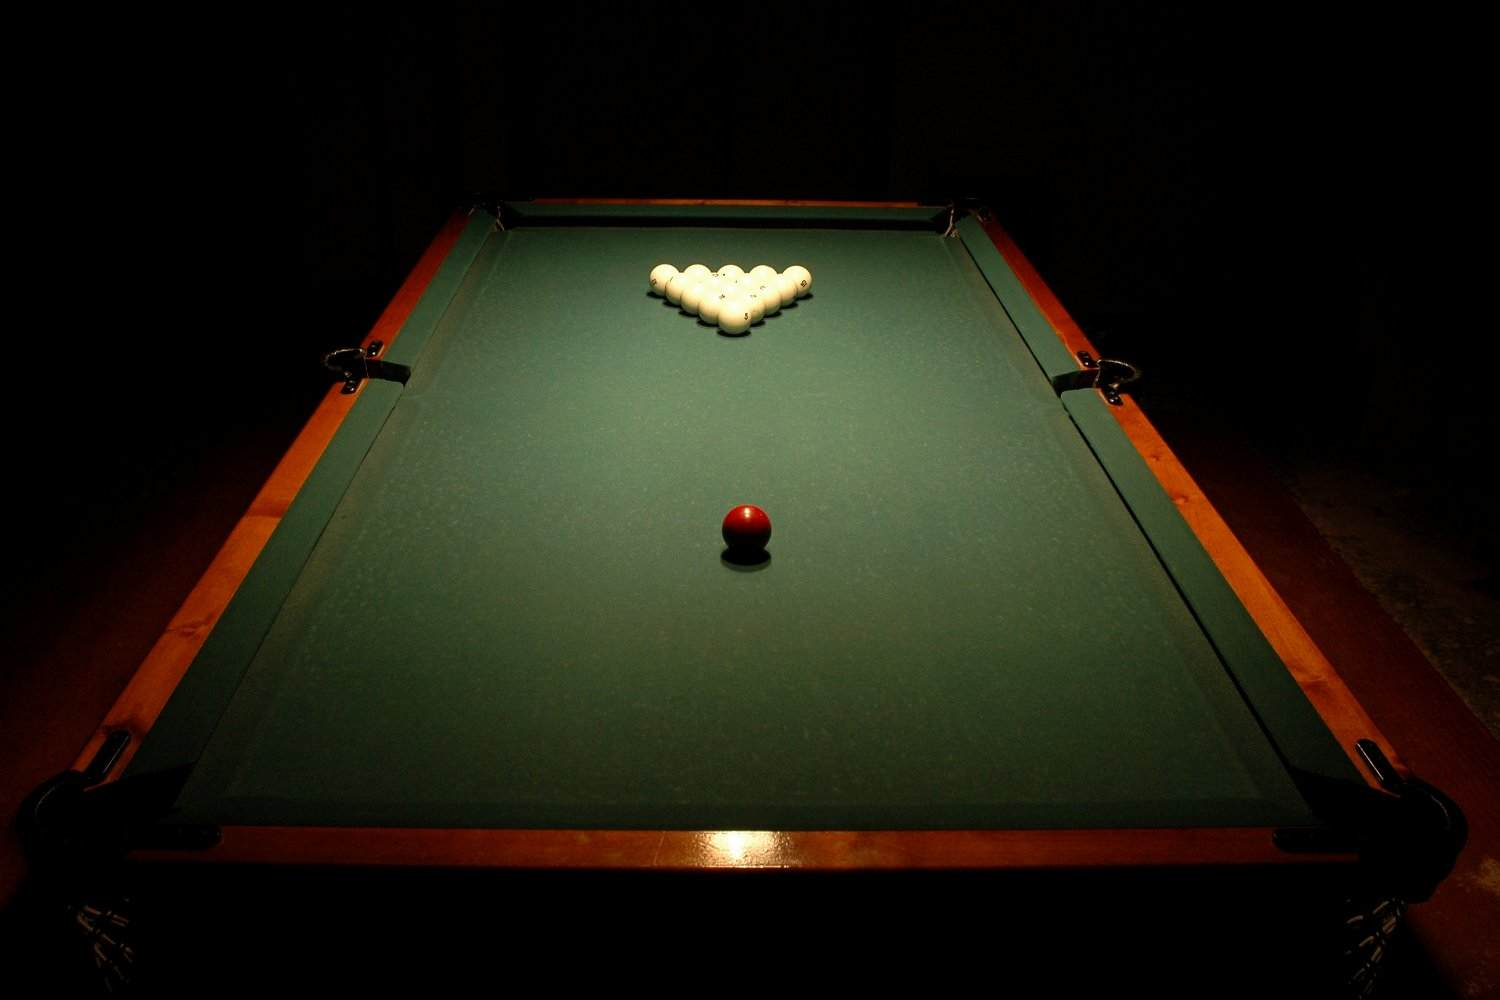
\includegraphics[width=3in]{billiards.jpg}
\end{figure}
\FloatBarrier
}


\begin{enumerate}

\easysubproblem How many ways is there to sink all balls if you assume at least one ball goes into each hole? \spc{3}

\easysubproblem How many ways is there to sink all balls if you do not assume at least one ball goes into each hole (i.e. pockets can be empty now)? \spc{3}

\hardsubproblem How many ways to sink all balls if pockets can be empty and the balls are distinct? \spc{3}

\extracreditsubproblem How many ways to sink all balls if pockets can be empty with the restriction that each pocket must have at least one odd ball and at least one even ball? \spc{8}

\extracreditsubproblem On the game in (b), let's say you win a special prize if the holes have three holes have 4 balls and the other three holes have one ball (4+4+4+1+1+1=12). You don't care which pockets have which balls but assume that each pocket has at least one ball. What is the probability you win this special prize upon sinking all balls? Assume that balls go into random pockets. Kind of silly... but it makes you think.  \spc{4}

\end{enumerate}

\problem Probability is rooted in gambling and thus we will be analyzing some gambling games. We will introduce the game of Roulette here. Basically, there's a ball that is dropped onto a spinning wheel with pockets for the ball to fall once the wheel and ball run out of momentum. There are 18 red pockets and 18 black pockets. There are two flavors of the game:

\begin{itemize}
\item European: There is one additional pocket colored green and labeled 0 (for a total of 18+18+1=37 pockets). An example of this wheel is pictured below on the left.
\item American: There are two additional pockets colored green labeled 0 and 00 (for a total of 18+18+2=38 pockets). An example of this wheel is pictured below on the right.
\end{itemize}

The gambler can make bets on any of the spaces as well as red (R), black (B), green (G), an odd number, an even number and a slew of other exotic type bets which we won't enumerate. We will be analyzing payoffs when we get to random variables next week but we will not be discussing them now.

\iftoggle{professormode}{
\begin{figure}[htp]
\centering
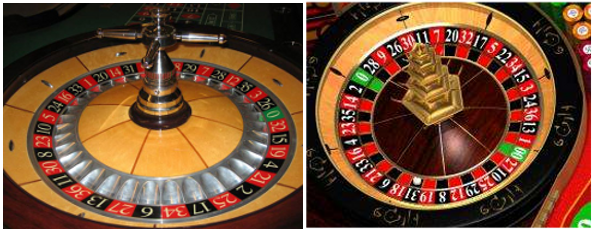
\includegraphics[width=4in]{roulette.png}
\end{figure}
\FloatBarrier
}

\begin{enumerate}
\easysubproblem What is the probability of the ball landing in a black pocket? Calculate for both European and American roulette.\spc{2}

\easysubproblem What is the probability of the ball landing in a green pocket? Calculate for both European and American roulette. \spc{2}

\easysubproblem What is the probability you see RRBBBRGRBB in 10 spins? \spc{2}

\easysubproblem In the 18 red pockets there are 9 even numbered pockets and 9 odd numbered pockets. What is the probability of getting a pocket wihich is both Red and Odd? \spc{2}

\easysubproblem What is the probability you see a spin that is both Red and Green? \spc{0.5}

\easysubproblem What is the probability you see a spin that is Red or Green? \spc{0.5}


\easysubproblem In America, you play the game 10 times and always bet on black. What is the probability you win all 10 times? \spc{2}

\hardsubproblem In America, you play the game 10 times and always bet on black. What is the probability you win at least once? \spc{2}

\end{enumerate}

\end{document}


%%%%%%%%%%%%%%%%%%%%%%%%%%%%%%%%%%%


\iftoggle{professormode}{
\paragraph{More counting} These counting questions will give you more practice in computing probabilities. Due to computations involving large factorials, we will also review Stirling's Approximation.\\ \\
}

\problem Imagine you have a bag of 10 cards where 6 are blue and 4 are red. A \qu{draw} means one card is taken out of the bag at random and the color is revealed. If the problem asks \qu{what is the probability,} this means an explicit computation is required unless otherwise stated.

\iftoggle{professormode}{
\begin{figure}[htp]
\centering
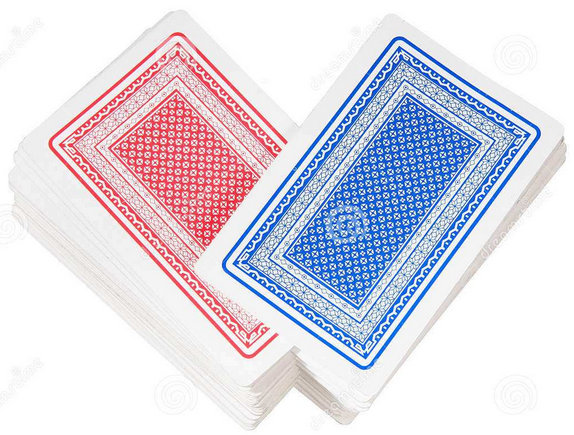
\includegraphics[width=2in]{red_blue.png}
\end{figure}
\FloatBarrier
}

\begin{enumerate}
\easysubproblem What is the probability of getting a blue card when drawing one card? \spc{1}

\easysubproblem What is the probability of drawing 3 red cards in a row \textit{without replacement}? \spc{1.5}

\intermediatesubproblem Five cards are drawn. What is the probability of having 3 reds and 2 blues without regards to any order of the cards? \spc{3.5}

\hardsubproblem Five cards are drawn. What is the probability of having 3 reds and 2 blues in that order? Think carefully about the numerator and denominator in this probability computation. \spc{3}

\intermediatesubproblem Five cards are drawn from a new bag with 100 cards where 60 are blue and 40 are red. What is the probability of having 3 reds and 2 blues without regards to any order of the cards? \spc{3.5}

\intermediatesubproblem Five cards are drawn from a new bag with 1000 cards where 600 are blue and 400 are red. What is the probability of having 3 reds and 2 blues without regards to any order of the cards? \spc{4}

\intermediatesubproblem Five cards are drawn from a new bag with $n$ cards where $0.6n$ are blue and $0.4n$ are red. What is the probability of having 3 reds and 2 blues without regards to any order of the cards? Do not compute the probability explicitly here; leave your solution as an algebraic expression \ie as a function of $n$. \spc{8.5}



\end{enumerate}

\problem Imagine you are putting together musical performances and you are employing musicians at random. There are many available for hire: 23 guitarists, 15 vocalists, 6 drummers, 14 bassists, 8 violinists, 9 violas, 6 cellists.


\iftoggle{professormode}{
\begin{figure}[htp]
\centering
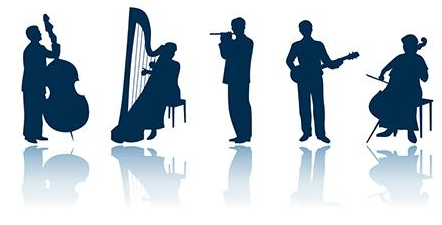
\includegraphics[width=2in]{musicians.png}
\end{figure}
\FloatBarrier
}

\begin{enumerate}
\easysubproblem If we hire 4 musicians at random, what is the probability we get a rock band (a vocalist, a guitarist, a bassist and a drummer)? \spc{3}

\easysubproblem If we hire 4 musicians at random, what is the probability we get a string quartet (two violinists, 1 cellist and one violist)? \spc{3}

\easysubproblem If we hire 4 musicians at random, what is the probability we get a doowop group (four vocalists)? \spc{7}

\easysubproblem We now move to a different city and the musicians for hire are different. Here, we have 10 guitarists, 10 vocalists, 10 drummers, 10 bassists. What is the probability we form a rock band when hiring four musicians at random? \spc{3}

\hardsubproblem Given the same situation in part (d), what is the probability we get two pairs of musicians (e.g. two guitarists and two bassists or two drummers and two bassists)? \spc{2.8}

\hardsubproblem Given the same situation in part (d), what is the probability we get all four musicians be the same type? \spc{3}

\end{enumerate}

\problem Computations of combinations and permutations is impossible for a computer due to the factorial computations. In this problem, we investigate Stirling's formula

\begin{enumerate}
\easysubproblem Use the natural log to derive an expression for $\binom{1500}{300}$ using sums. \spc{3}

\easysubproblem The logs in the previous problem would allow us to compute. What would be a downside? \spc{1}


\easysubproblem Show that Stirling's approximation is equivalent to the expression I wrote in class:

\beqn
\natlog{n!} \approx \half\natlog{2\pi} + \parens{n + \half}\natlog{n} - n
\eeqn
\spc{5}

\hardsubproblem Use the expression in (c) to approximate the probability of getting 300 Heads in 1500 coin flips. \spc{6}

\end{enumerate}

\problem Combinations are not only useful in probability problems. They come up all over mathematics.

\begin{enumerate}
\intermediatesubproblem In the first lecture we mentioned that $\abss{2^\Omega} = 2^{|\Omega|}$. (recall that the powerset contains all subsets of $\Omega$ \ie $A \in 2^\Omega~~\forall A \subseteq \Omega$). We reasoned that each $\omega \in \Omega$ can be either \textit{in} or \textit{out} of a subset. Thus on/off for the first outcome, on/off for the second outcome, etc. to make 2 raised to the number of elements. This will count every possibly subset. All \qu{offs} would result in $\varnothing$ and all \qu{ons} will result in $\Omega$. 

Assume $\Omega = \braces{a,b,c,d}$. Explain \textit{in English} how the following equation is true by explaining each element in the sum.

\beqn
\abss{2^\Omega} = \sum_{i=0}^{|\Omega|} \binom{|\Omega|}{i}
\eeqn

It may be helpful to draw out $2^\Omega$ explicitly and write out the above equation in order to see the pattern. Each of the combination terms will correspond to a subset of $2^\Omega$. \spc{6}

\easysubproblem  Recall the binomial theorem:

\beqn
(a + b)^n = \sum_{i=0}^n \binom{n}{i} a^{n-i} b^i
\eeqn

Explain \textit{in English} why are the $\binom{n}{i}$ terms called \qu{binomial coefficients.} \spc{2.5}


\extracreditsubproblem Prove the equality in part (a) for arbitrary but finite-sized $\Omega$. \spc{9}

\extracreditsubproblem Prove the binomial expansion in part (b) for arbitrary $n \in \naturals$. \spc{9}

\end{enumerate}



\iftoggle{professormode}{
\paragraph{Philosophy of Probability} Problems below are related to the readings in Gillies as well as the material we covered in class. The link to Gillies' book is in on the first page of this PDF.\\ \\ 
}

\problem Answer the following questions by writing a paragraph or two \textit{in English}.

\begin{enumerate}
\easysubproblem Which definition of probability does the book use and why do you think the authors chose this definition? \spc{4}

\easysubproblem  Give an example of an event whose probability cannot be approximated by the limiting frequency. \spc{1.5}

\intermediatesubproblem Give an example of a random event involving an object's \qu{propensity} and explain this definition of probability. \spc{2.5}

\easysubproblem Discuss the difference between the \qu{logical} and the \qu{subjective} definition of probability. \spc{4.5}


\easysubproblem Explain the difference between \qu{objective} and \qu{epistemic} interpretations of probability. Which definitions fall under these categories? Classify all four of Gillies' definitions in this way. \spc{3.5}


\extracreditsubproblem For the objective definitions where experiments are conducted, who picks $\omega \in \Omega$ \ie the outcome from the set of possible outcomes in the universe? Discuss your thoughts. \spc{4.5}

%\extracreditsubproblem Is probability an illusion or is it real? Is randomness a fundamental property of the universe? Discuss your thoughts. \spc{10}

\end{enumerate}

\problem We will be looking into the long term frequency definition here. For this problem, you must have \texttt{R} installed. Please download it from \url{http://cran.r-project.org/} (there are links for Windows, MAC and Linux) and then double-click to open an \texttt{R} console.

\begin{enumerate}

\easysubproblem To calculate combinations, use the \texttt{choose(n,k)} function. Calculate the number of five-card hands from a standard deck by copying the following code into \texttt{R} and then pressing enter:

\begin{knitrout}
\begin{kframe}
\begin{verbatim}
choose(52, 5)
\end{verbatim}
\end{kframe}
\end{knitrout}

Please write down the answer. Is the answer the same as we computed in class? \spc{2.5}

\easysubproblem Verify the probability in class of a ``full house'' by copying the following code into \texttt{R} and then pressing enter:

\begin{knitrout}
\begin{kframe}
\begin{verbatim}
choose(13, 1) * choose(4, 3) * choose(12, 1) * choose(4, 2) / 
  choose(52, 5)
\end{verbatim}
\end{kframe}
\end{knitrout}

Write down the answer as a \textit{percentage}. \spc{3.5}

\intermediatesubproblem We are going to do a little experiment to explore the definition of probability as a limiting frequency. We will be looking at the context of flipping a coin and getting heads. Remember the definition was

\beqn
\prob{\braces{H}} = \limitn \frac{\displaystyle \sum_{i=1}^n \indic{\omega_i \in \braces{H}}}{n}
\eeqn

(where $\indic{T}$ is the \qu{indicator function} which equals 1 when the expression $T$ is true and 0 if the expression $T$ is false). We will run a simulation with large values of $n$. Copy and paste the following code into your \texttt{R} terminal:

\begin{knitrout}
\begin{kframe}
\begin{verbatim}
N = 30000
sims = sample(0:1, N, replace = T)
freqs_by_n = array(NA, N)
for (n in 1 : N){
  freqs_by_n[n] = sum(sims[1:n]) / n
}
plot(10:N, 
  freqs_by_n[10:N], 
  xlim = c(10, N), 
  ylim = c(0.40, 0.60), 
  pch = ".", 
  xlab = "number of samples",
  ylab = "frequency of heads",
  main = "P(H) as a limiting frequency: 30,000 samples")
abline(h = 0.5, col = "blue")
freqs_by_n[N]
#last line placeholder
\end{verbatim}
\end{kframe}
\end{knitrout}

\inred{If the code throws an error, download the PDF to your computer and try copying and pasting again. It does NOT work from a browser window. The PDF must be downloaded.}

The console should have popped up a plot.\footnote{This is a \textit{real} statistical simulation. Each time you run this code it will be different. You can compare plots with your friends but take note that they will not look exactly the same.} Print this out and attach it to your homework. If you are using \LaTeX, you can include the figure into the PDF.

From the title of the plot and the x and y axes, tell a story about what is going on here \textit{in English}. \spc{3.5}

\easysubproblem What is the limiting frequency of heads after 30,000 coin flips to 3 decimals based on the simulation in the previous problem? (that is the number that appears in the console directly after ``\texttt{$>$ freqs\_by\_n[N]}'') \spc{1.5}

\end{enumerate}

\end{document}
